\copyrightVincent

\updatehighlight{
	name=accentC,
	remove={},
	add={equation},
	%
	name=default,
	add={}
}

\begin{saveblock}{equation}
	\begin{highlightblock}[gobble=8,linewidth=\textwidth,
		framexleftmargin=0.25em,xleftmargin=0.25em]
		De trigonometrische identiteit is
		$ \sin^2(\theta) + \cos^2(\theta) = 1 $.

		De trigonometrische identiteit is 
		\begin{equation}
			\sin^2(\theta) + \cos^2(\theta) = 1.
		\end{equation}
	\end{highlightblock}
\end{saveblock}

\begin{saveblock}{equationEN}
	\begin{highlightblock}[gobble=8,linewidth=\textwidth,
		framexleftmargin=0.25em,xleftmargin=0.25em]
		The trigonometric identity is
		$ \sin^2(\theta) + \cos^2(\theta) = 1 $.

		The trigonometric identity is
		\begin{equation}
			\sin^2(\theta) + \cos^2(\theta) = 1.
		\end{equation}
	\end{highlightblock}
\end{saveblock}

% Daarmee kunnen we de
% verdubbelingsformule herschrijven
% als
% \begin{align}
% 	\cos(2\theta) 
% 	&= \cos^2(\theta) 
% 		- \sin^2(\theta)\\
% 	&= 2\cos^2(\theta)-1.
% \end{align}

\addtorecentlist{equation}

\begin{frame}{Equation}
	\useblock{equation\langsuffix}

	\includegraphics[width=\linewidth,height=0.4\textheight,keepaspectratio]{%
		assets/mathEquation\langsuffix.pdf}

	% \begin{columns}
	% 	\begin{column}{0.6\textwidth}
	% 		\useblock{equation}
	% 	\end{column}
	% 	\begin{column}{0.5\textwidth}
	% 		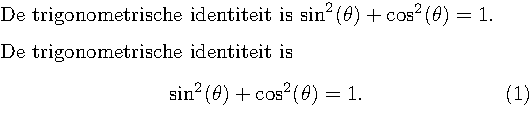
\includegraphics[width=\linewidth,height=0.8\textheight,keepaspectratio]{assets/mathEquation.pdf}
	% 	\end{column}
	% \end{columns}
\end{frame}

\updatehighlight{
	name=accentC,
	remove={equation},
	%
	name=default,
	add={}
}
